%!TEX root = ../thesis-main.tex

\chapter{Conclusioni}
Quanto discusso nell'elaborato nel suo complesso ha consentito la distribuzione del software Alchemist in modo automatico in formati standard delle piattaforme coinvolte, le quali rappresentano due famiglie di sistemi operativi completamente differenti. Gli obiettivi posti sono stati raggiunti grazie ad una valutazione degli strumenti adibiti alla pacchettizzazione che il panorama \ac{jvm} offre, e grazie all'utilizzo di tecnologie come Gradle e GitHub Actions, sono state integrate all'interno del flusso di integrazione e distribuzione continua del progetto. L'autovalutazione ha poi evidenziato l'ottimo risultato ottenuto rispetto l'iniziale flusso di integrazione utilizzato nel progetto.

\begin{figure}[htb]
	\centering
	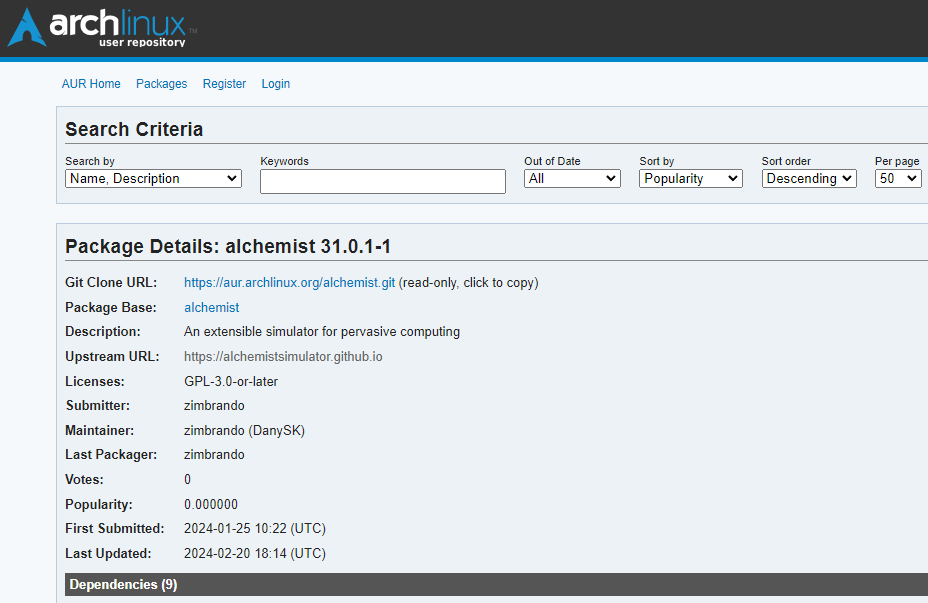
\includegraphics[width=.8\linewidth]{figures/alchemist-aur.png}
	\caption{Pagina web raffigurante il pacchetto Alchemist pubblicato sul repository AUR}
	\label{fig:aur-web}
\end{figure}

Il conseguimento degli obiettivi è osservabile su GitHub nella sezione dei rilasci\footnote{https://github.com/AlchemistSimulator/Alchemist/releases}, dove è possibile notare la possibilità di scaricare i diversi pacchetti installanti per ogni sistema operativo. Mediante invece l'utilizzo dei package manager è possibile installare ed aggiornare Alchemist con l'utilizzo di un semplice comando. Su Windows, previa installazione di winget, attraverso:
\texttt{winget install Unibo.alchemist}
e su Arch e derivate, previa autorizzazione all'installazione dall'Arch User Repository\footnote{https://aur.archlinux.org/packages/alchemist}(\Cref{fig:aur-web}), tramite \texttt{pamac} per Manjaro o più generalmente \texttt{yay}.
L'utilizzo dei package manager assicura all'utente l'installazione dell'ultima versione di Alchemist e mediante le funzionalità da questo offerte è altrettanto semplice aggiornare la sua versione, in modo da garantire l'utilizzo agli utenti delle ultime funzionalità del simulatore. 

\section{Sviluppi futuri}
L'implementazione descritta da questo elaborato ha aperto nuove possibilità di distribuzione del progetto mediante l'introduzione della pacchettizzazione. Attraverso lo sviluppo di processi automatici di pubblicazione il software è stato distribuito all'interno di due principali repository di riferimento. Le possibilità di estensione del progetto sono numerose, in quanto esistono molteplici package manager nel panorama esteso dei sistemi operativi. Nei seguenti punti sono riassunti i principali spunti per migliorare ed estendere il processo:
\begin{itemize}
	\item \textbf{Distribuzione su Homebrew}: i repository su cui Alchemist è distribuito non comprendono il sistema operativo MacOs. Il package manager Homebrew realizzato per MacOs rappresenta una valida opzione per raggiungere un pubblico più ampio attraverso modalità di installazione semplici e funzionali.
	\item \textbf{Supporto a Snap}: un'altra tipologia, nell'ambiente Linux, sono i pacchetti detti containerizzati, ovvero eseguiti all'interno di ambienti separati con un accesso limitato al sistema. Questa caratteristica fornisce due principali vantaggi: la possibilità per una applicazione di usare la propria versione desiderata di librerie di sistema senza creare conflitti e la trasparenza all'utente nell'accesso alle risorse di sistema, garantendo quindi un livello aggiuntivo di sicurezza. È il caso dei pacchetti \textit{snap}, pacchetti self-contained considerati universali perché compatibili con una notevole quantità di distribuzioni Linux. La loro implementazione nel flusso di integrazione e distribuzione continua di Alchemist contribuirebbe ad un ulteriore ampliamento delle distribuzioni supportate dal software. 
\end{itemize}
